\section{Hardware Design: Efficient Architecture}\label{sec:hardware}

In this section, we investigate the hardware level techniques used in state-of-the-art FPGA-based neural network accelerator design to achieve high performance and high energy efficiency. We classify the techniques into three levels: computation unit level, loop unrolling level, and system level.

\subsection{Computation Unit Designs}\label{sec:hardware:cu}

Computation unit level design affects the peak performance of the neural network accelerator. The available resource of an FPGA chip is limited. A smaller computation unit design means more computation units and higher peak performance. A carefully designed computation unit array can also increase the working frequency of the system and thus improve peak performance.

\subsubsection{Low Bit-width Computation Unit}\label{sec:hardware:cu:lbu}
Reduce the number of bit-width for computation is a direct way to reduce the size of computation units. The feasibility of using fewer bits comes from the quantization methods as introduced in section~\ref{sec:software:quant}. Most of the state-of-the-art FPGA designs replace the 32-bit floating-point units with fixed-point units. Podili et al.~\cite{podili2017fast} implement 32-bit fixed-point units for the proposed system. 16-bit fixed-point units are widely adopted in \cite{qiu2016going, li2016high, xiao2017exploring, guan2017fp, zhang2016caffeine}. ESE~\cite{han2017ese} adopts 12-bit fixed-point weight and 16-bit fixed-point neurons design. Guo et al.~\cite{guo2017angel} use 8-bit units for their design on embedded FPGA. Recent work is also focusing on extremely narrow bit-width design. Prost-Boucle et al.~\cite{prost2017scalable} implements 2-bit multiplication with 1 LUT for ternary networks. Experiments in \cite{nurvitadhi2016accelerating} show that FPGA implementation of Binarized Neural Network (BNN) outperforms that on CPU and GPU. Though BNN suffers from accuracy loss, many designs explore the benefit of using 1-bit data for computation~\cite{li20177, nakahara2017batch, zhao2017accelerating, umuroglu2017finn, nakahara2017fully, jiao2017accelerating, moss2017high, yang2018fully, ghasemzadehrebnet}.

The designs mentioned above focus on computation units for linear quantization. For non-linear quantization, translating the data back to full precision for computation still costs many resources. Samragh et al.~\cite{samragh2017customizing} propose the factorized coefficients based dot product implementation. As the possible values of weights are quite limited for non-linear quantization, the proposed computation unit accumulates the multipliers for each possible weight value and calculate the result as the weighted sum of the values in look-up tables. In this way, the multiplication needed for one output neuron equals to the number of values in look-up table. The multiplications are replaced by random-addressed accumulations.

Most of the designs use one bit-width through the process of a neural network. Qiu et al.~\cite{qiu2016going} finds that neurons and weights in FC layers can use fewer bits compared with CONV layers while the accuracy is maintained. Heterogeneous computation units are used in the designs of \cite{zhao2017accelerating, guo2017bit}.

The size of computation units of different bit-widths is compared in Table~\ref{tab:mac}. Three kinds of implementations are tested: separate multiplier and adder with logic resource on Xilinx FPGA, multiply-add function with DSP units on Xilinx FPGA, and multiply-add function with DSP units on Altera FPGA. The resource consumption is the synthesis result by Vivado 2018.1 targeting Xilinx XCKU060 FPGA and Quartus Prime 16.0 targeting Altera Arria 10 GX1150 FPGA. The pure logic modules and the floating-point multiply and add modules are generated with IP core. The fixed-point multiply and add modules are implemented with $A*B+C$ in Verilog and automatically mapped to DSP by Vivado/Quartus.

We first give an overview of the size of the computation units by logic-only implementations. By compressing the weights and activations from 32-bit floating-point number to 8-bit fixed-point number, the multiplier and the adder are scaled down to about 1/10 and 1/50 respectively. Using 4-bit or smaller operators can bring further advantage but also incur significant accuracy loss as introduced in section~\ref{sec:software:quant}. 

Recent FPGAs consist of a large number of DSP units, each of which implements hard multiplier, pre-adder and accumulator core. The basic pattern of NN computation, multiplication and sum, also fits into this design. So we also test the multiply and add function implemented with DSP units. Because of the different DSP architectures, we test on both Xilinx and Altera platforms. Compared with the 32-bit floating-point function, fixed-point functions with narrow bit-width still shows an advantage in resource consumption. But for Altera FPGA, this advantage is not obvious because the DSP units natively support floating-point operations. 

Fixed-point functions with 16-or-less-bit fixed-point data are well fit into 1 DSP unit on either Xilinx or Altera FPGA. This shows that quantization hardly benefits the hardware if we use narrower bit-width like 8 or 4 in the aspect of computation. The problem is that the wide multipliers and adders in DSP units are underutilized in these cases. Nguyen et al.~\cite{nguyen2017double} propose the design to implement two narrow bit-width fixed-point multiplication with a single wide bit-width fixed-point multiplier. In this design, two multiplications, $AB$ and $AC$, are executed in the form of $A(B<<k+C)$. If $k$ is sufficiently large, the bits for $AB$ and $AC$ does not overlap in the multiplication result and can be directly separated. The design in~\cite{nguyen2017double} implements two 8-bit multiplications with one $25\times 18$ multiplier, where $k$ is 9. Similar methods can be applied to other bit-width and DSPs.

%\begin{figure}[ht]
%    \centering
%    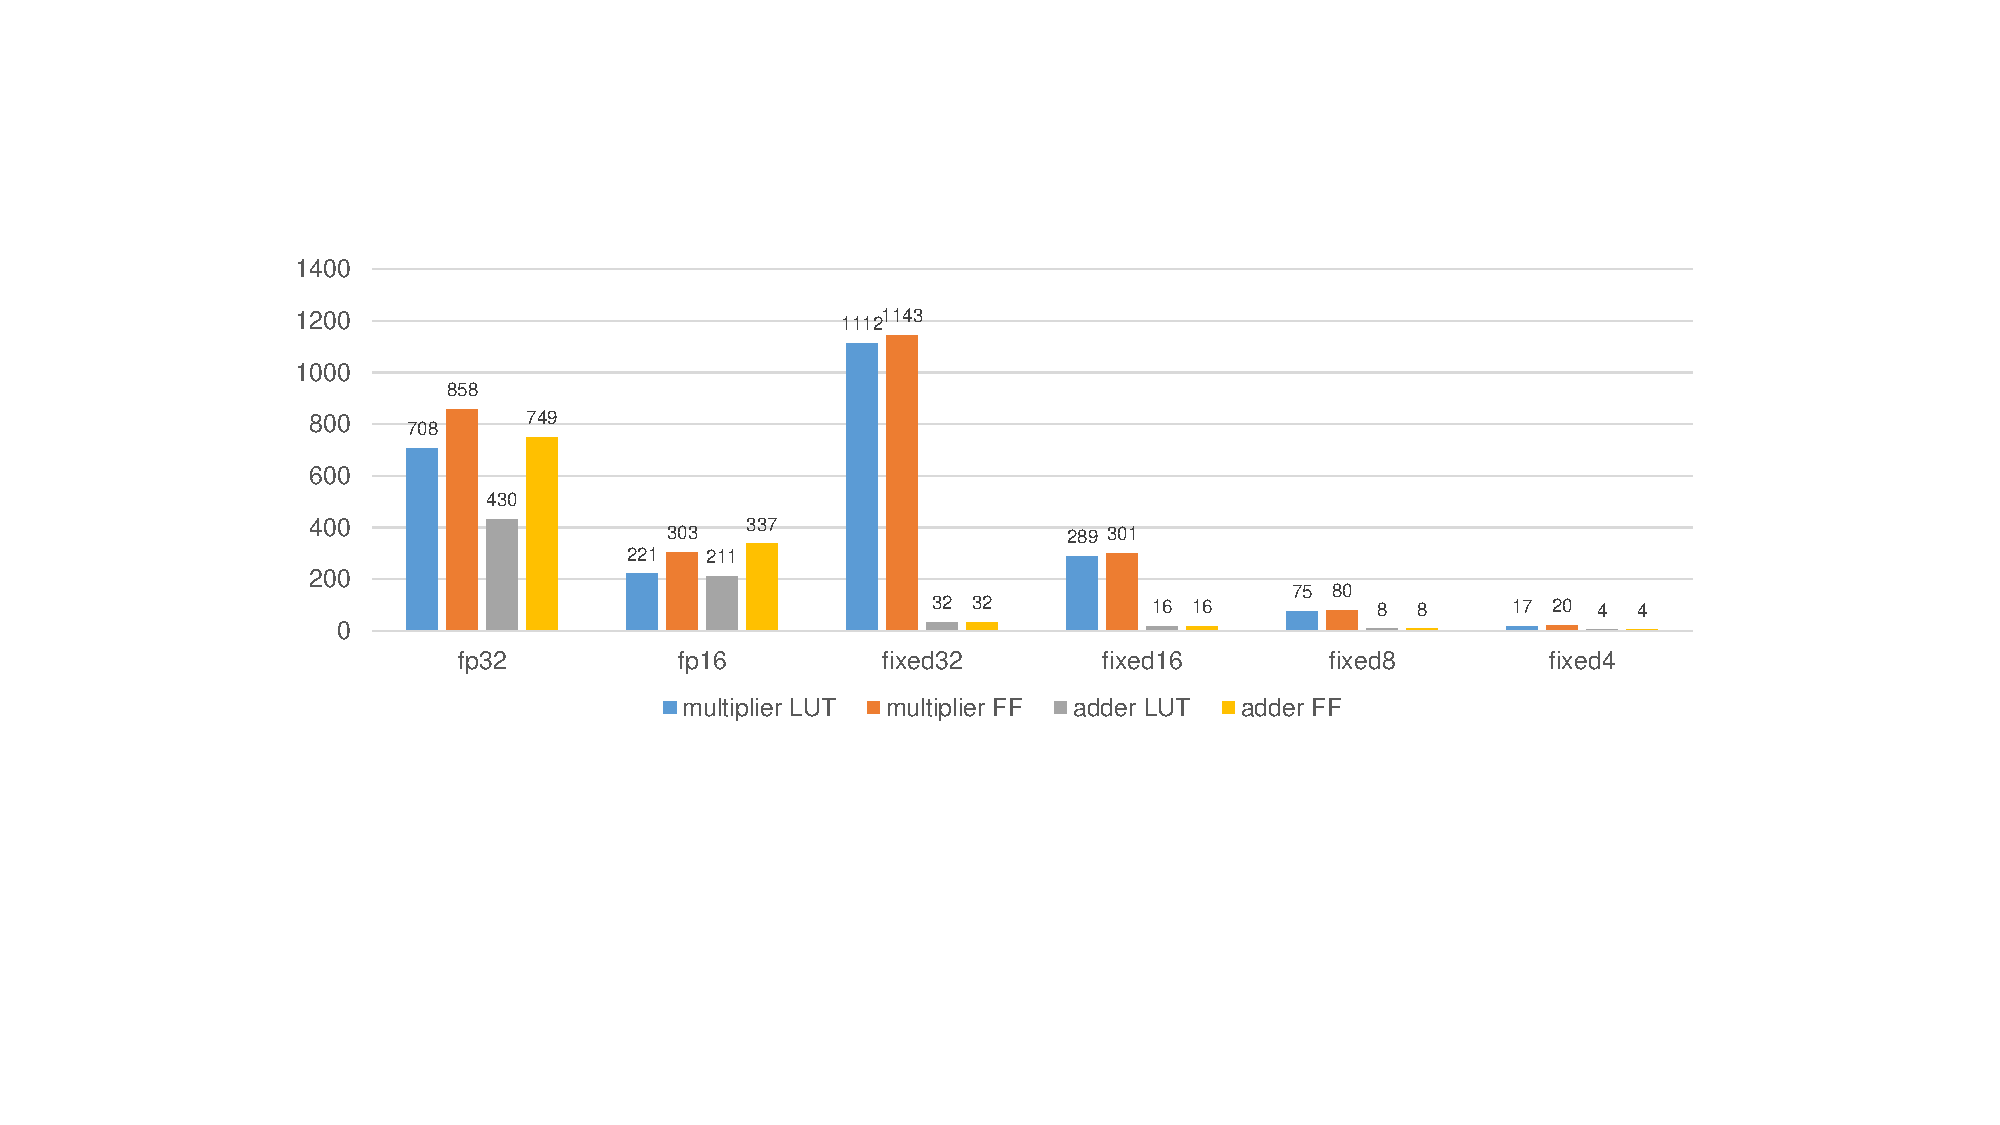
\includegraphics[width=1.0\columnwidth]{fig/mac_util.pdf}
%    \caption{FPGA resource consumption comparison for multiplier and adder with different types of data.}
%    \label{fig:mac_util}
%\end{figure}

% Table generated by Excel2LaTeX from sheet 'Sheet1'
\begin{table}[htbp]
    \centering
    \caption{\rev{FPGA resource consumption comparison for multiplier and adder with different types of data.}}
      \begin{tabular}{|l|r|r|r|r|r|r|r|r|r|} \hline
      \multirow{2}[4]{*}{} & \multicolumn{4}{c|}{Xilinx Logic} & \multicolumn{3}{c|}{Xilinx DSP} & \multicolumn{2}{c|}{Altera DSP} \\ \cline{2-10}         
       & \multicolumn{2}{c|}{multiplier} & \multicolumn{2}{c|}{adder} & \multicolumn{3}{c|}{multiply \& add} & \multicolumn{2}{c|}{multiply \& add} \\ \cline{2-10}
            & \multicolumn{1}{c|}{LUT} & \multicolumn{1}{c|}{FF} & \multicolumn{1}{c|}{LUT} & \multicolumn{1}{c|}{FF} & \multicolumn{1}{c|}{LUT} & \multicolumn{1}{c|}{FF} & \multicolumn{1}{c|}{DSP} & \multicolumn{1}{c|}{ALM} & \multicolumn{1}{c|}{DSP} \\ \hline
      fp32  & 708   & 858   & 430   & 749   & 800   & 1284  & 2     & 1     & 1 \\ \hline
      fp16  & 221   & 303   & 211   & 337   & 451   & 686   & 1     & 213   & 1 \\ \hline
      fixed32 & 1112  & 1143  & 32    & 32    & 111   & 64    & 4     & 64    & 3 \\ \hline
      fixed16 & 289   & 301   & 16    & 16    & 0     & 0     & 1     & 0     & 1 \\ \hline
      fixed8 & 75    & 80    & 8     & 8     & 0     & 0     & 1     & 0     & 1 \\ \hline
      fixed4 & 17    & 20    & 4     & 4     & 0     & 0     & 1     & 0     & 1 \\ \hline
      \end{tabular}
    \label{tab:mac}
  \end{table}
  

\subsubsection{Fast Convolution Method}\label{sec:hardware:cu:fcu}
For CONV layers, the convolution operations can be accelerated by alternative algorithms. Discrete Fourier Transformation (DFT) based fast convolution is widely adopted in digital signal processing. Zhang et al.~\cite{zhang2017frequency} propose a 2D DFT based hardware design for efficient CONV layer execution. For an $F\times F$ filter convolved with $K\times K$ filter, DFT converts the $(F-K+1)^2K^2$ multiplications in the space domain to $F^2$ complex multiplications in the frequency domain. For a CONV layer with $M$ input channel and $N$ output channel, $MN$ times of frequency domain multiplications and $(M+N)$ times DFT/IDFT are needed. The conversion of convolution kernels is once for all. So the domain conversion process is of low cost for CONV layers. This technique does not work for CONV layers with stride>1 or $1\times 1$ convolution. Ding et al.~\cite{ding2017c} suggest that a block-wise circular constraint can be applied to the weight matrix. In this way, the matrix-vector multiplication in FC layers are converted to a set of 1D convolutions and can be accelerated in the frequency domain. This method can also be applied to CONV layers by treating the $K\times K$ convolution kernels as $K\times K$ matrices and is not limited by $K$ or stride.

Frequency domain methods require complex number multiplication. Another kind of fast convolution involves only real number multiplication~\cite{winograd1980arithmetic}. The convolution of a 2D feature map $F_{in}$ with a kernel $K$ using Winograd algorithm is expressed by equation~\ref{eqt:winograd}.
\begin{equation}\label{eqt:winograd}
    F_{out} = A^T[(GF_{in}G^T)\odot(BF_{in}B^T)]A
\end{equation}
$G$, $B$ and $A$ are transformation matrix which only related to the sizes of kernel and feature map. $\odot$ denotes an element-wise multiplication of two matrices. For a $4\times 4$ feature map convolved with a $3\times 3$ kernel, the transformation matrices are described as follows:
\begin{equation*}
    G = \left[
        \begin{array}{ccc}
            1           & 0            & 0           \\
            \frac{1}{2} & \frac{1}{2}  & \frac{1}{2} \\
            \frac{1}{2} & -\frac{1}{2} & \frac{1}{2} \\
            0           & 0            & 1
        \end{array}    
    \right] \quad
    B = \left[
        \begin{array}{cccc}
            1 & 0  & -1 & 0 \\
            0 & 1  & 1  & 0 \\
            0 & -1 & 1  & 0 \\
            0 & 1  & 0  & -1
        \end{array}
    \right] \quad
    A = \left[
        \begin{array}{cc}
            1 & 0  \\
            1 & 1  \\
            1 & -1 \\
            0 & -1 
        \end{array}
    \right]
\end{equation*}
Multiplication with transformation matrices $A, B$ and $G$ induce only a small number of shift and addition because of the special matrix entries. In this case, the number of multiplication is reduced from 36 to 16.The most commonly used Winograd transformation is for $3\times 3$ convolutions in \cite{lu2017evaluating, xiao2017exploring}. 

The theoretical performance gain from fast convolution depends on the convolution size. Limited by the on-chip resource and the consideration of flexibility, current designs are not choosing large convolution sizes. Existing work point out that up to $4\times$ theoretical performance gain can be achieved by fast convolution with FFT~\cite{zhang2017frequency} or Winograd~\cite{lu2017evaluating} with reasonable kernel sizes. Zhuge et al.~\cite{zhuge2018face} even try to use both FFT and Winograd methods in their design to fit different kernel sizes in different layers.

\subsubsection{Frequency Optimization Methods}
All the above techniques introduced targets at increasing the number of computation units within a certain FPGA. Increasing the working frequency of the computation units also improves the peak performance.

Latest FPGAs support 700-900MHz DSP theoretical peak working frequency. But existing designs usually work at 100-400MHz~\cite{qiu2016going, guo2017angel, zhang2016caffeine, ma2017optimizing, zhang2017improving}. As claimed in \cite{wu2017high}, the working frequency is limited by the routing between on-chip SRAM and DSP units. The design in \cite{wu2017high} uses different working frequencies for DSP units and surrounding logic. Neighbor slices to each DSP unit are used as local RAMs to separate the clock domain. The prototype design in \cite{wu2017high} achieves the peak DSP working frequency at 741MHz and 891MHz on FPGA chips of different speed grades. \rev{Xilinx has also proposed the CHaiDNN-v2~\cite{chai_dnn} and xfDNN~\cite{xfdnn} with this technique and achieves up to 700MHz DSP working frequency. Compared with existing designs for which the frequency is within 300MHz, this technique brings at least $2\times$ peak performance gain.}

\subsection{Loop Unrolling Strategies}\label{sec:hardware:lu}
CONV layers and FC layers contribute to most of the computations and storage requirement of a neural network as introduced in section~\ref{sec:preliminary}. We express the CONV layer function in Figure~\ref{fig:cnn_preliminary}(b) as nested loops in Algorithm~\ref{alg:conv}. To make the code clear to read, we merge the loops along $x$ and $y$ directions for feature maps and 2-D convolution kernels respectively. An FC layer can be expressed as a CONV layer with feature map and kernel both of size $1\times 1$. Besides the loops in Algorithm~\ref{alg:conv}, we also call the parallelism of the process of multiple inputs as a batch. As we treat FC layers and CONV layers all as nested loops, the loop unrolling strategy can be applied both in CNN accelerators and RNN accelerators. But as the case for FC layers are rather simple, we tend to use CNN as examples in this section.

\begin{algorithm}  
    \caption{Convolution Layer}
    \label{alg:conv}
    \begin{algorithmic}[1]
        \Require feature map $F_{in}$ of size $M\times Y\times X$; 
                 convolution kernel $Ker$ of size $N\times M\times K\times K$;
                 bias vector $b$ of size $N$ 
        \Ensure  feature map $F_{out}$
        \Function {ConvLayer}{$F_{in}, Ker$}  
            \State Let $F_{out} \gets $ zero array of size $N\times(Y-K+1)\times(X-K+1)$  
            \For{$n=1$; $n<N$; $n++$} \Comment Output channel loop
                \For{$m=1$; $m<M$; $m++$} \Comment Input channel loop
                    \For{each $(y, x)$ within $(Y-K+1, X-K+1)$} \Comment Feature map loop
                        \For{each $(ky, kx)$ within $(K, K)$} \Comment Kernel loop
                            \State $F_{out}[n][y][x] += F_{in}[m][y-ky+1][x-kx+1] * K[n][m][ky][kx]$
                        \EndFor
                    \EndFor
                \EndFor
                \State $F_{out}[n] += b[n]$
            \EndFor
            \State \Return{$F_{out}$}
        \EndFunction  
        
    \end{algorithmic}  
\end{algorithm}

\subsubsection{Choosing Unroll Parameters}

To parallelize the execution of the loops, we unroll the loops and parallelize the process of a certain number of iterations on hardware. The number of the parallelized iterations on hardware is called the unroll parameter. Inappropriate unroll parameter selection may lead to serious hardware underutilization. Take a single loop as an example. Suppose the trip count of the loop is $M$ and the parallelism is $m$. The utilization ratio of the hardware is limited by $m/M\lceil M/m\rceil$. If $M$ is not divisible by $m$, then the utilization ratio is less than 1. For processing an NN layer, the total utilization ratio will be the product of the utilization ratio on each of the loops.

%Take an example of three nested loops as shown in Figure~\ref{fig:unrolling}. The big cube denotes all the operations within the loops. The length of each edge denotes the trip count of each loop. The small cube denotes the unrolled kernel. The hardware process all the operations of a small cube in parallel. To finish the workload, the hardware computes the small cubes one by one.  Figure~\ref{fig:unrolling}(a) shows an appropriate set of unroll parameters. But for Figure~\ref{fig:unrolling}(b), the red part of some of the small cubes are out of the big cube, which means the hardware is wasted.

%\begin{figure}[ht]
%    \centering
%    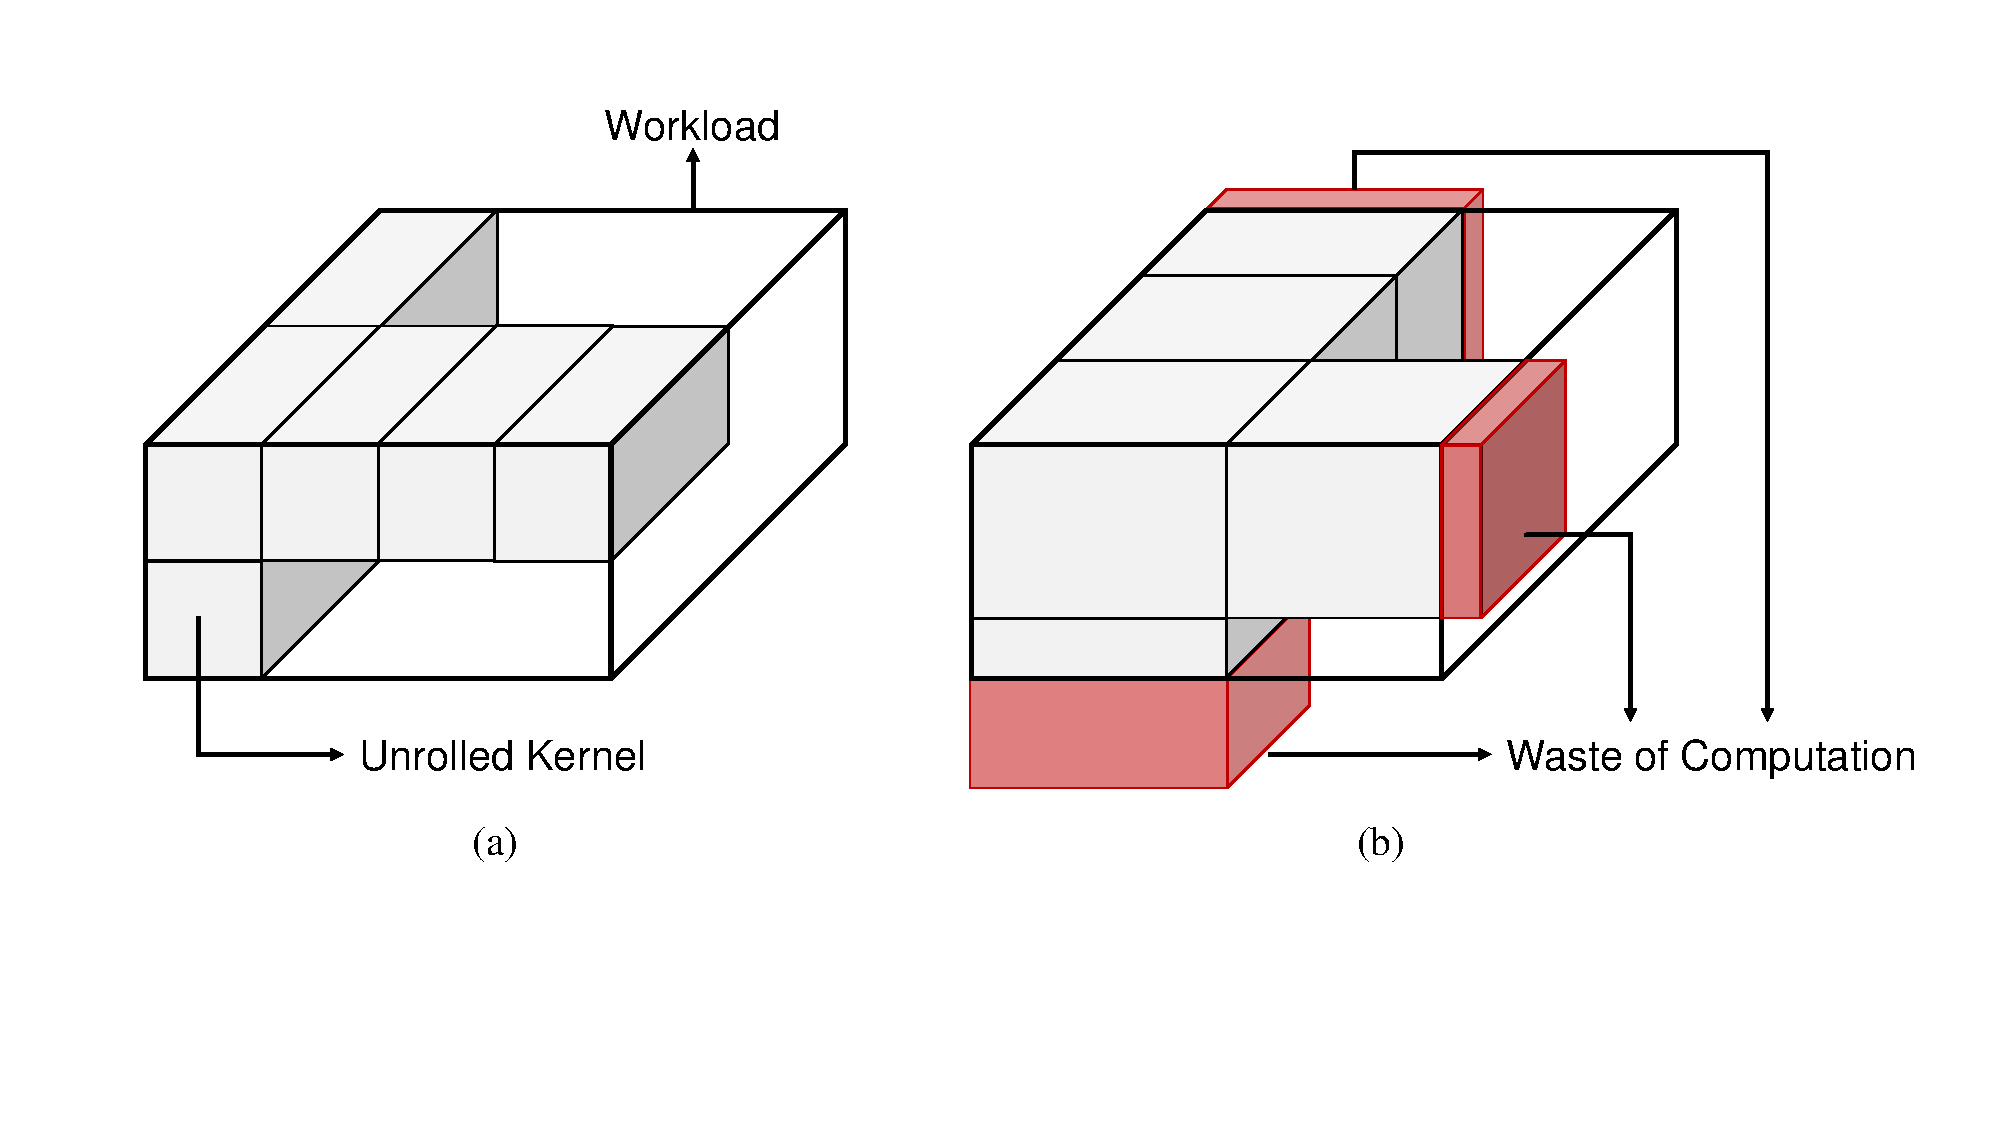
\includegraphics[width=0.8\columnwidth]{fig/unrolling.pdf}
%    \caption{Comparison between appropriate and inappropriate loop unroll parameters. (a) Appropriate parameters. (b) Inappropriate parameters.}
%    \label{fig:unrolling}
%\end{figure}

For a CNN model, the loop dimension varies greatly among different layers. For a typical network used on ImageNet classification like ResNet~\cite{he2016deep}, the channel numbers vary from 3 to 2048; the feature map sizes vary from $224\times 224$ to $7\times 7$, the convolution kernel sizes vary from $7\times 7$ to $1\times 1$. Besides the underutilization problem, loop unrolling also affect the datapath and on-chip memory design. Thus loop unrolling strategy is a key feature for a neural network accelerator design. 

Various work are proposed focusing on how to choose the unroll parameters. Zhang et al.~\cite{zhang2015optimizing} propose the idea of unrolling the input channel and output channel loops and choose the optimized unroll parameter by design space exploration. Along these two loops, there is no input data cross-dependency between neighboring iterations. So no multiplexer is needed to route data from the on-chip buffer to computation units. But the parallelism is limited as $7\times 64=448$ multipliers. For larger parallelism, this solution is easy to suffer from the underutilization problem. Ma et al.~\cite{ma2017optimizing} further extends the design space by allowing parallelism on the feature map loop. The parallelism reaches $1\times 16\times 14\times 14=3136$ multipliers. A shift register structure is used to route feature map pixels to the computation units.

The kernel loop is not chosen in the above work because kernel sizes vary greatly. Motamedi et al~\cite{motamedi2016design} use kernel unrolling on AlexNet. Even with $3\times 3$ unrolling for the $11\times 11$ and $5\times 5$ kernels, the overall system performance still reaches 97.4\% of its peak performance for the convolution layers. For certain networks like VGG~\cite{simonyan2014very}, only $3\times 3$ convolution kernels are used. Another reason to unroll kernel loop is to achieve acceleration with fast convolution algorithms. Design in \cite{zhang2017frequency} implements fully parallelized frequency domain multiplication on $4\times 4$ feature map and $3\times 3$ kernel. Lu et al.~\cite{lu2017evaluating} implement Winograd algorithm on FPGA with a dedicated pipeline for equation~\ref{eqt:winograd}. The convolution of a $6\times 6$ feature map with a $3\times 3$ kernel is fully parallelized.

The above solutions are only for a single layer. But there is hardly a one-size-fits-all solution for a whole network, especially when we need high parallelism. Designs in \cite{li2016high, liu2016automatic, zhang2018dnnbuilder} propose fully pipelined structures with each layer a pipe stage. As each layer is executed with an independent part of the hardware and each part is small, loop unrolling method can be easily chosen. This method is memory consuming because ping-pong buffers are needed between adjacent layers for the feature maps. Agressive design with binarized weights~\cite{yang2018fully} can fit into FPGA better. Design in \cite{zhang2016energy} is similar but implemented on FPGA clusters to resolve the scalability problem. Shen et al.~\cite{shen2016overcoming} and Lin et al.~\cite{lin2018lcp} group the layers of a CNN by the loops' trip count and map each group onto one hardware module. These solutions can be treated as unrolling the batch loop because different inputs are processed in parallel on different layer pipeline stages. The design in \cite{lu2017evaluating} implements parallelized batch both within a layer and among different layers. 

Most of the current designs follow one of the above methods for loop unrolling. A special kind of design is for sparse neural networks. Han et al.~\cite{han2017ese} propose the ESE architecture for sparse LSTM network acceleration. Unlike processing a dense network, all the computation units will not work synchronously. This causes difficulty in sharing data between different computation units. ESE implements only the output channel (the output neurons of the FC layers in LSTM) loop unrolling within a layer to simplify hardware design and parallelize batch process.

\subsubsection{Data Transfer and On-chip Memory Design}

Besides the high parallelism, the on-chip memory system should efficiently offer the necessary data to each computation units every cycle. To implement high parallelism, neural network accelerators usually reuse data among a large number of computation units. Simply broadcasting data to different computation units leads to large fan-out and high routing cost and thus reduce the working frequency. Wei et al.~\cite{wei2017automated} use the systolic array structure in their design. The shared data are transferred from one computation unit to the next in a chain mode. So the data is not broadcasted, and only local connections between different computation units are needed. The drawback is the increase in latency. The loop execution order is scheduled accordingly to cover the latency. Similar designs are adopted in~\cite{aydonat2017opencl, ma2017optimizing}. 

For software implementation on GPU, the im2col function is commonly used to map 2D convolution as a matrix-vector multiplication. This method incurs considerable data redundancy and can hardly be applied to the limited on-chip memory of FPGAs. Qiu et al.~\cite{qiu2016going} uses the line buffer design to achieve the $3\times 3$ sliding window function for 2-d convolution with only two lines of duplicated pixels. 

\subsection{System Design}\label{sec:hardware:sys}

A typical FPGA-based neural network accelerator system is shown in Figure~\ref{fig:sys}. The logic part of the whole system is denoted by the blue boxes. The host CPU issues workload or commands to the FPGA logic part and monitors its working status. On the FPGA logic part, a controller is usually implemented to communicate with the host and generates control signals to all the other modules on FPGA. The controller can be an FSM or an instruction decoder. The on the fly logic part is implemented for certain designs if the data loaded from external memory needs preprocess. This module can be data arrangement module, data shifter~\cite{qiu2016going}, FFT module~\cite{zhang2017frequency}, etc. The computation units are as discussed in section~\ref{sec:hardware:cu} and section~\ref{sec:hardware:lu}. As introduced in section~\ref{sec:preliminary:fpga}, on-chip SRAM of an FPGA chip is too limited compared with the large NN models. So for common designs, a two-level memory hierarchy is used with DDR and on-chip memory. 

\begin{figure}[t]
    \centering
    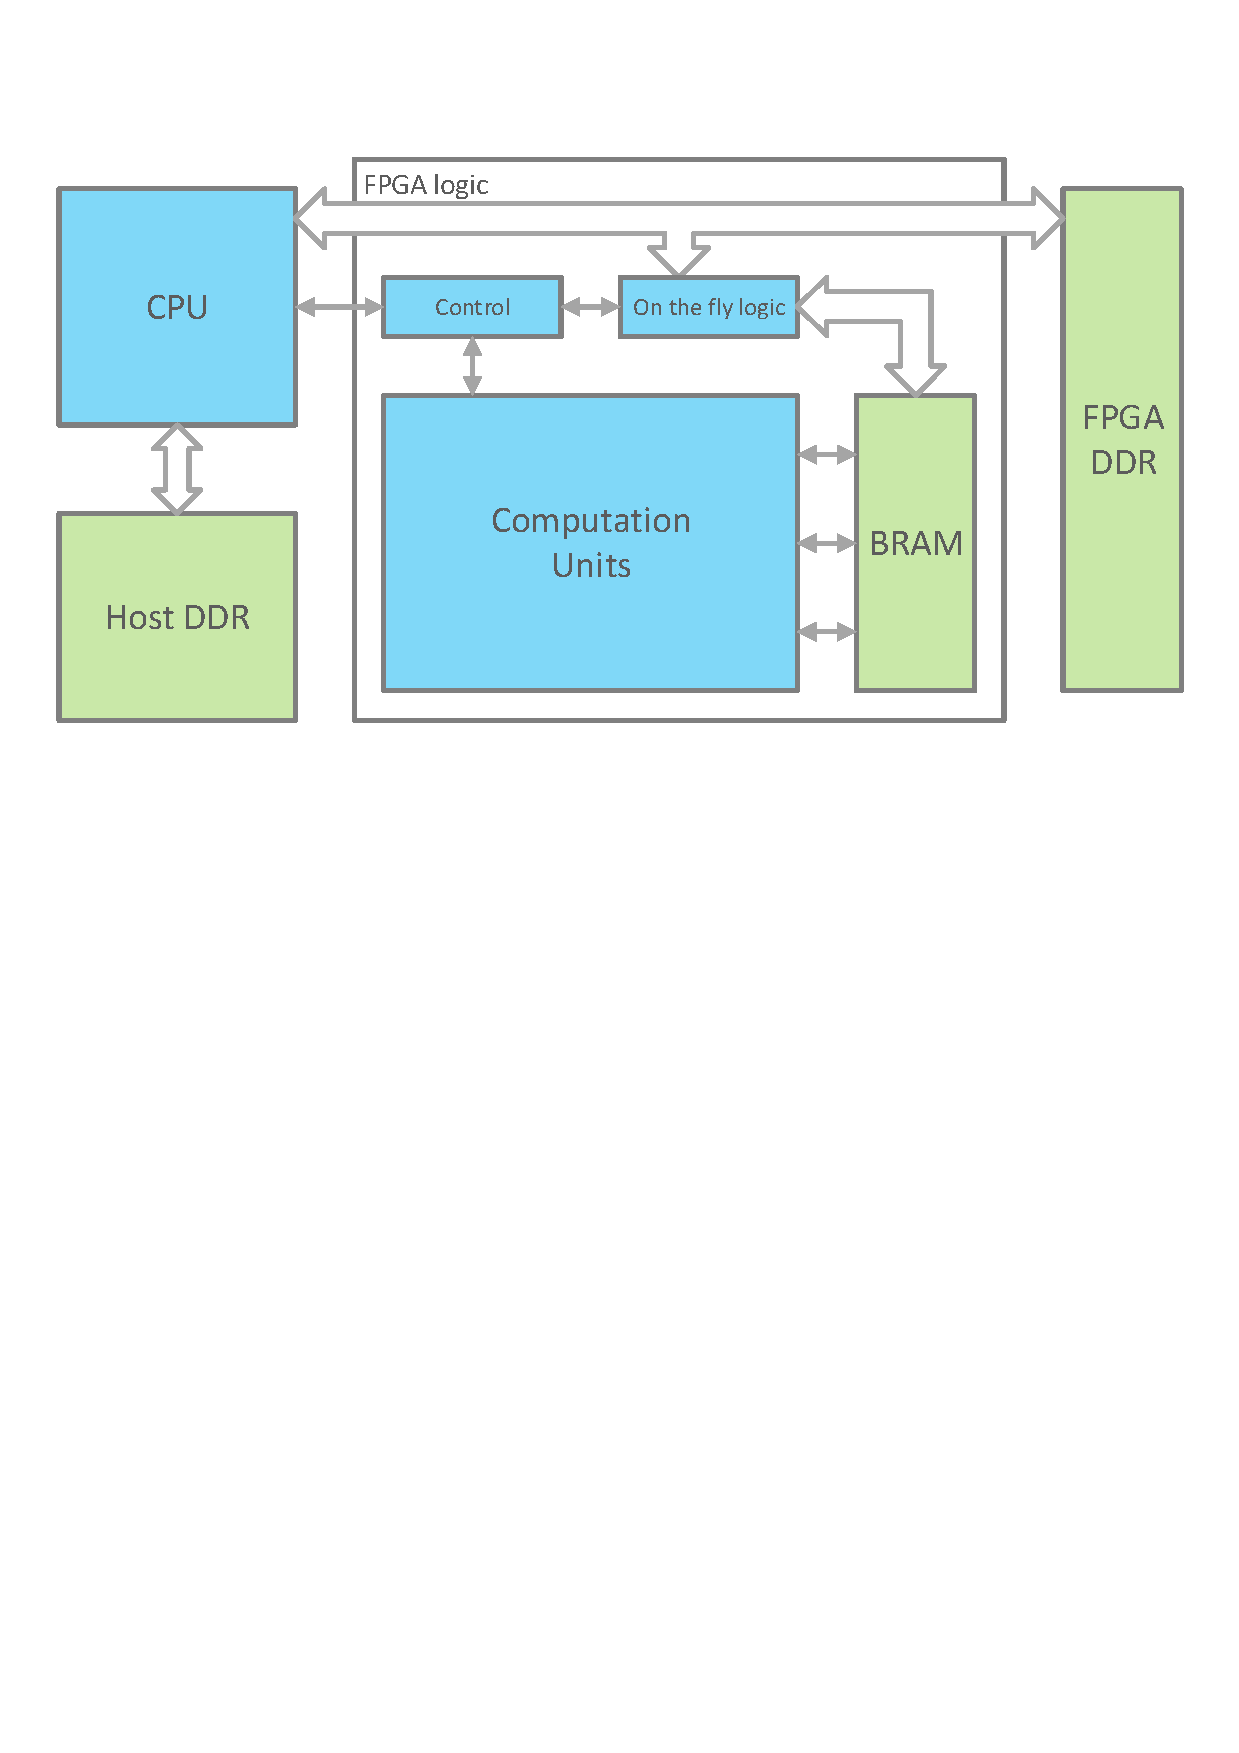
\includegraphics[width=0.8\columnwidth]{fig/sys.pdf}
    \caption{Block graph of a typical FPGA-based neural network accelerator system}
    \label{fig:sys}
\end{figure}

\subsubsection{\rev{Roofline Model}} From the system level, the performance of a neural network accelerator is limited by two factors: the on-chip computation resource and the off-chip memory bandwidth. Various researches have been proposed to achieve the best performance within a certain off-chip memory bandwidth. Zhang et al.~\cite{zhang2015optimizing} introduce the roofline model in their work to analyze whether a design is memory bounded or computation bounded. An example of a roofline model is shown in Figure~\ref{fig:roofline}.

\begin{figure}[h]
    \centering
    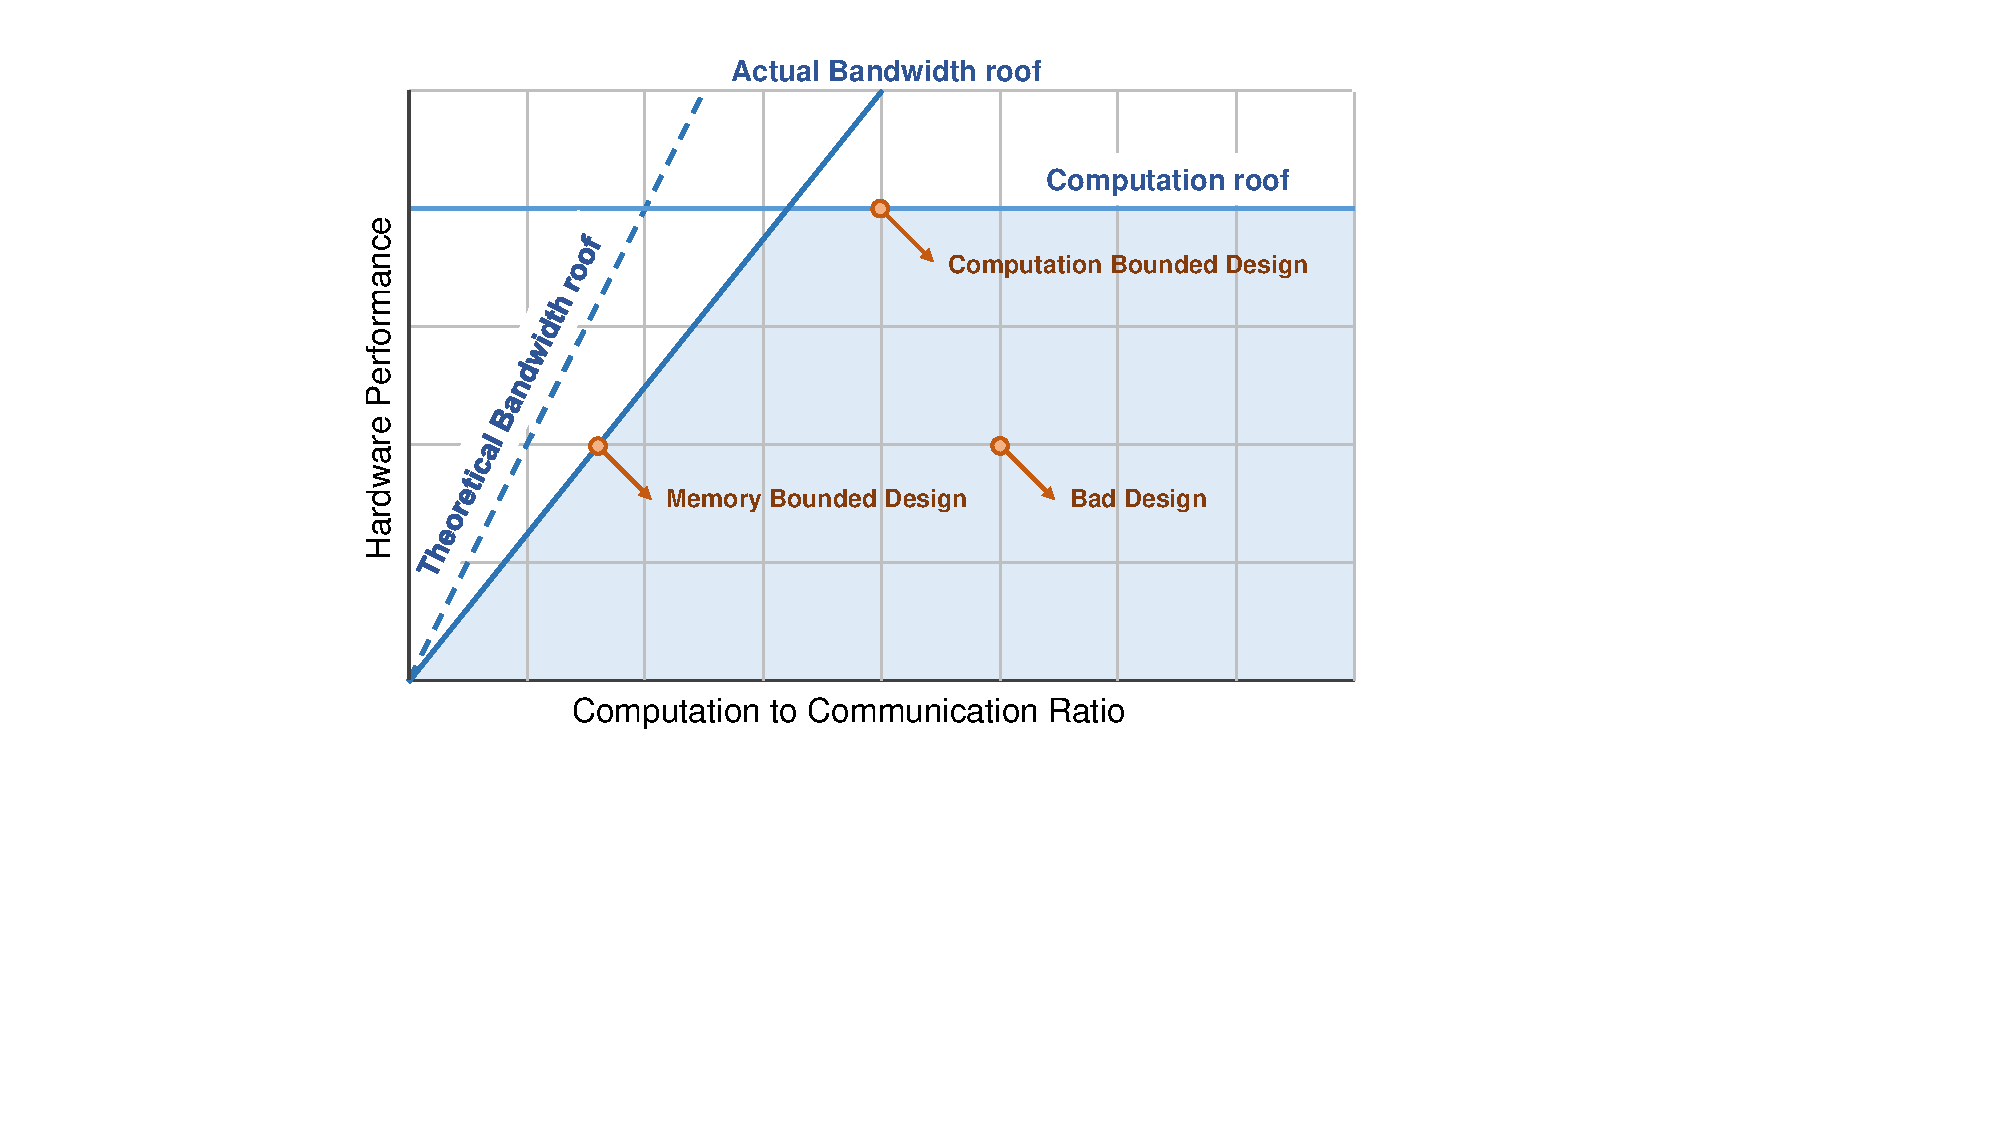
\includegraphics[width=0.6\columnwidth]{fig/roofline.pdf}
    \caption{An example of the roofline model. The shaded part denotes the valid design space given bandwidth and resource limitation.}
    \label{fig:roofline}
\end{figure}

The figure uses the computation to communication (CTC) ratio as the $x$-axis and hardware performance as the $y$-axis. CTC is the number of operations that can be executed with a unit size of memory access. Each hardware design can be treated as a point in the figure. So $y/x$ equals to the bandwidth requirement of the design. The available bandwidth of a target platform is limited and can be described as the theoretical bandwidth roof in Figure~\ref{fig:roofline}. But the actual bandwidth roof is below the theoretical roof because the achievable bandwidth of DDR depends on the data access pattern. Sequential DDR access achieves much higher bandwidth than random access. The other roof is the computation roof, which is limited by the available resource on FPGA.

\subsubsection{\rev{Loop Tiling and Interchange}} A higher CTC ratio means the hardware is more likely to achieve the computation bound. Increasing the CTC ratio also reduce DDR access, which significantly saves energy according to~\cite{vlsi_energy}. In section~\ref{sec:hardware:lu}, we have discussed the loop unrolling strategies to increase the parallelism while reducing the waste of computation for a certain network. When the loop unrolling strategy is decided, the scheduling of the rest part of the loops decides how the hardware can reuse data with on-chip buffer. This involves loop tiling and loop interchange strategy.

Loop tiling is a higher level of loop unrolling. All the input data of a loop tile will be stored on-chip, and the loop unrolling hardware kernel works on these data. A larger loop tile size means that each tile will be loaded from external memory to on-chip memory fewer times. Loop interchange strategy decides the processing order of the loop tiles. External memory access happens when the hardware is moving from one tile to the next. Neighboring tile may share a part of data. For example in a CONV layer, neighboring tile can share input feature map or the weights. This is decided by the execution order of the loops. 

In ~\cite{zhang2015optimizing, ma2017optimizing}, design space exploration is done on all the possible loop tiling sizes and loop orders. Many designs also explore the design space with some of the loop unrolling, tiling and loop order is already decided~\cite{motamedi2016design, qiu2016going}. Shen et al.~\cite{shen2017escher} also discuss the effect of batch parallelism over the CTC for different layers. This is a loop dimension not focused on in previous work.

All the above work give one optimized loop unrolling strategy and loop order for a whole network. Guo et al.~\cite{guo2017angel} implements flexible unrolling and loop order configuration for different layers with an instruction interface. The data arrangement in on-chip buffers is controlled through instructions to fit with different feature map sizes. This means the hardware can always fully utilize the on-chip buffer to use the largest tiling size according to on-chip buffer size. This work also proposes the "back and forth" loop execution order to avoid total on-chip data refresh when an innermost loop finishes.

\subsubsection{\rev{Cross-Layer Scheduling}} Alwani et al.~\cite{alwani2016fused} address the external memory access problem by fusing two neighboring layers together to avoid the intermediate result transfer between the two layers. This strategy helps reduce 95\% off-chip data transfer with extra 20\% on-chip memory cost. Even software program gains $2\times$ speedup with this scheduling strategy. Yu et al.~\cite{Yu2017Instruction} realize this idea on a single-layer accelerator design by modifying the order of execution through an instruction interface.

\subsubsection{\rev{Regularize Data Access Pattern}} Besides increasing CTC, increasing the actual bandwidth roof helps improve the achievable performance with a certain CTC ratio. This is achieved by regularizing the DDR access pattern. The common feature map formats in the external memory include $NCHW$ or $CHWN$, where $N$ means the batch dimension, $C$ means the channel dimension, $H$ and $W$ means the feature map $y$ and $x$ dimension. Using any of these formats, a feature map tile may be cut into small data blocks stored in discontinuous addresses. Guan~\cite{guan2017fp} suggest that a channel-major storage format should be used for their design. This format avoids data duplication while long DDR access burst is ensured. Qiu et al.~\cite{qiu2016going} propose a feature map storage format that arranges the $H\times W$ feature map into $(HW/rc)$ tile blocks of size $r\times c$. So the write burst size can be increased from $c/2$ to $rc/2$.
